\section{A planar coordinate and a uniform slice estimate}
\label{sec:planar}

We use Gross's conformal map $\psi$ for the uniform distribution
\cite[Section~3.2]{Gross2019}, with the rotation $F(w)=i\psi(iw)$.
There is no scaling. The same lens appears in
\cite[Section~3]{SymmetricCompanion2026}; its half-width $\lambda(t)$
is the function $V(t)$ used here. We establish its needed properties
directly and then prove a uniform slice estimate that controls the
momentum coordinates in the polar product.

\begin{lemma}\label{lem:planar-map}
The holomorphic function
\begin{equation}\label{eq:planar-F}
 F(w)=\frac{8}{\pi^2}\sum_{\ell=0}^{\infty}
       \frac{(-1)^\ell w^{2\ell+1}}{(2\ell+1)^2},
 \qquad w\in\D,
\end{equation}
is a biholomorphism from \(\D\) onto a bounded domain \(D\).
It is odd, commutes with conjugation, and satisfies \(F(0)=0\).
The imaginary coordinates of \(D\) range over \((-1,1)\), and for each
\(t\in(-1,1)\) there is a finite \(V(t)>0\) such that
\begin{equation}\label{eq:horizontal-slices}
 \{v\in\R:v+it\in D\}=(-V(t),V(t)).
\end{equation}
Write \(F(ir)=iT(r)\) for \(0\le r<1\).  The function \(T\) increases
strictly from \(0\) to \(1\), with
\begin{equation}\label{eq:planar-T}
 T'(r)=\frac{8}{\pi^2}\frac{\operatorname{arctanh}r}{r}
 \quad(0<r<1),
 \qquad \lim_{r\uparrow1}T'(r)=+\infty.
\end{equation}
For fixed \(t\in(-1,1)\), put \(r_0=T^{-1}(|t|)\).  The positive
horizontal slice is parametrized by
\[
 w(r,t)=re^{i\theta(r,t)},\qquad
 F(w(r,t))=v(r,t)+it,\qquad r_0<r<1,
\]
where \(-\pi/2<\theta(r,t)<\pi/2\) and \(v(r,t)\) increases strictly
from \(0\) to \(V(t)\).
\end{lemma}

\begin{proof}
\noindent\textit{The map and its angular derivative.}
The series in Equation~\eqref{eq:planar-F} is absolutely summable on the
closed disk.  Hence \(F\) is bounded, odd, and commutes with conjugation.
Termwise differentiation in the open disk gives
\begin{equation}\label{eq:planar-arctan}
 wF'(w)=\frac{8}{\pi^2}\arctan w,
 \qquad
 \arctan w=\frac{1}{2i}\log\frac{1+iw}{1-iw}.
\end{equation}
Here the logarithm is the branch on the right half-plane that is real on
the positive real axis.  Indeed,
\[
 \Re\frac{1+iw}{1-iw}
   =\frac{1-|w|^2}{|1-iw|^2}>0
 \qquad (w\in\D).
\]
This also shows that \(\arctan w=0\) only at \(w=0\).
Thus \(F'\) has no zeros away from the origin, and the series gives
\(F'(0)=8/\pi^2\ne0\).

For \(w=re^{i\theta}\), define
\begin{equation}\label{eq:planar-A}
 A(r,\theta)=\Re\bigl(wF'(w)\bigr)
   =\frac{4}{\pi^2}
       \arctan\frac{2r\cos\theta}{1-r^2}.
\end{equation}
To obtain the last identity, the imaginary part of the fraction in
Equation~\eqref{eq:planar-arctan}, divided by its real part, is
\(2r\cos\theta/(1-r^2)\), and its argument lies in
\((-\pi/2,\pi/2)\).  On the right semicircle,
\(0<A(r,\theta)<2/\pi\).  The identities
\begin{equation}\label{eq:planar-polar-derivatives}
 \partial_r F(re^{i\theta})=\frac{wF'(w)}{r},
 \qquad
 \partial_\theta F(re^{i\theta})=iwF'(w)
\end{equation}
therefore show that \(\Re F(w)>0\) in the right half-disk: its radial
derivative is positive, and its value tends to zero at the origin.
They also show that \(\Im F(re^{i\theta})\) increases strictly with
\(\theta\) on each right semicircle.

Oddness and conjugation symmetry give \(F(ir)=iT(r)\) with real \(T\).
Differentiating Equation~\eqref{eq:planar-arctan} on the imaginary axis
gives Equation~\eqref{eq:planar-T}.  In particular, \(T\) is strictly
increasing, \(T(0)=0\), and \(T'(r)\) diverges as \(r\uparrow1\).
Since \(F(r)\) is real, Equation~\eqref{eq:planar-polar-derivatives}
also gives
\[
 T(r)=\int_0^{\pi/2}A(r,\theta)\,d\theta.
\]
The integrand is bounded by \(2/\pi\) and tends to \(2/\pi\) at every
\(\theta\in[0,\pi/2)\) as \(r\uparrow1\).  Dominated convergence
therefore gives \(T(r)\to1\).

\medskip
\noindent\textit{Horizontal slices and global invertibility.}
Fix \(|t|<1\) and let \(T(r_0)=|t|\).  For every \(r\in(r_0,1)\),
the strictly increasing imaginary coordinate on the right semicircle
ranges from \(-T(r)\) to \(T(r)\).  There is consequently exactly one
angle \(\theta(r,t)\) there with imaginary coordinate \(t\).
It depends smoothly on \(r\), since its angular derivative is \(A>0\).
Writing \(wF'(w)=A+iB\), implicit differentiation at fixed \(t\) gives
\[
 \partial_r\theta=-\frac{B}{rA},
 \qquad
 \partial_r v=\frac{A}{r}-B\,\partial_r\theta
             =\frac{A^2+B^2}{rA}.
\]
Thus
\begin{equation}\label{eq:horizontal-radius-derivative}
 \frac{\partial v}{\partial r}(r,t)
   =\frac{|wF'(w)|^2}{rA(r,\theta(r,t))}>0.
\end{equation}
As \(r\downarrow r_0>0\), the angle tends to the appropriate imaginary-axis
endpoint of the semicircle, so \(v(r,t)\to0\).  If \(r_0=0\), the same
limit follows from \(F(0)=0\).  Boundedness of \(F\) now shows that
\(v(r,t)\) maps \((r_0,1)\) continuously and strictly increasingly onto
an interval \((0,V(t))\), where \(0<V(t)<\infty\).

This parametrization proves injectivity on each positive horizontal
slice.  The reflection identity
\(F(-\overline w)=-\overline{F(w)}\) gives the negative slices, and the
strict monotonicity of \(T\) gives injectivity on the imaginary axis.
The right half-disk, imaginary axis, and left half-disk have images with
positive, zero, and negative real parts, respectively.  Hence \(F\) is
globally injective.  Every point of its image has imaginary coordinate
in \((-1,1)\), and every such coordinate occurs on the imaginary axis.
This proves Equation~\eqref{eq:horizontal-slices}.  Since \(F'\ne0\),
the local holomorphic inverses combine into a holomorphic inverse
\(g:D\to\D\).
\end{proof}

Figure~\ref{fig:lens-slices} illustrates the radial parametrization of a
horizontal slice.  Along the right half of the highlighted disk curve,
\(\Im F(w)=t\) stays fixed while \(|w|\) increases, and its image moves
to the right along the horizontal slice.
Equation~\eqref{eq:horizontal-radius-derivative} therefore allows us to
rewrite horizontal integrals using the disk radius \(r\), as we do below.
\begin{figure}[htb]
  \centering
  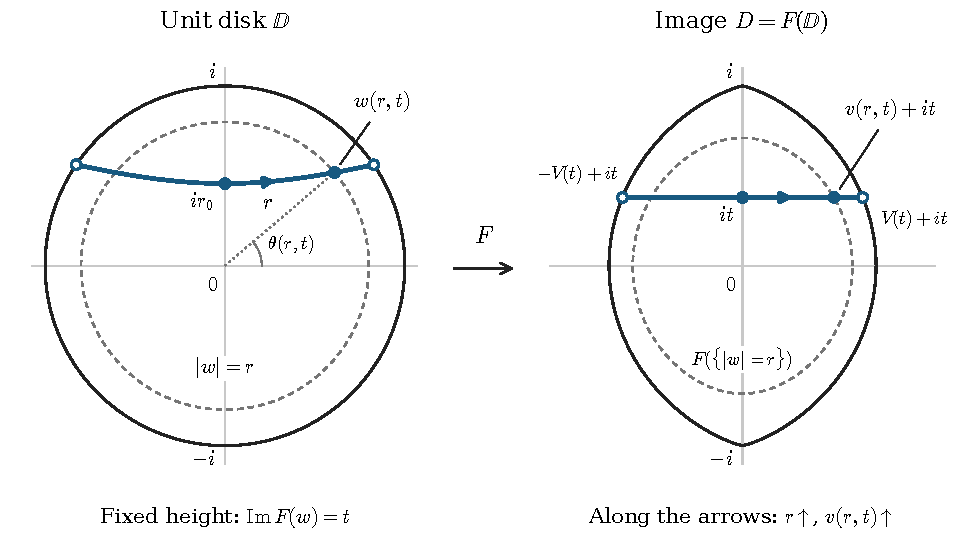
\includegraphics[width=\linewidth]{figures/lens-slices.pdf}
  \caption{A fixed horizontal slice and its preimage, illustrated for $t>0$.
  Along the right half of the highlighted preimage curve in the left panel,
  $r$ increases from
  $r_0=T^{-1}(t)$ to $1$, while $v(r,t)$ increases from $0$ to $V(t)$.
  The dashed circle and its image pass through the corresponding marked
  points. Open markers indicate boundary limits.}
  \label{fig:lens-slices}
\end{figure}


For an integer \(k\ge2\), define the signed slice integral
\begin{equation}\label{eq:slice-primitive}
 J_k(v,t)=k^2\int_0^v
       |g(h+it)|^{2k-2}|g'(h+it)|^2\,dh,
 \qquad v+it\in D.
\end{equation}
The segment of integration lies in \(D\) by Lemma~\ref{lem:planar-map}.

\begin{proposition}\label{prop:uniform-slice}
Each \(J_k\) is smooth on \(D\), is odd in \(v\), and satisfies
\begin{equation}\label{eq:slice-derivative}
 \partial_v J_k(v,t)
    =k^2|g(v+it)|^{2k-2}|g'(v+it)|^2\ge0.
\end{equation}
There is a sequence \(\epsilon_k\ge0\), depending only on \(F\), with
\(\epsilon_k\to0\) such that, simultaneously for every \(v+it\in D\),
\begin{equation}\label{eq:uniform-slice}
 \frac{|J_k(v,t)|}{k}
    \le\frac{\pi}{4}|g(v+it)|^{2k}+\epsilon_k.
\end{equation}
\end{proposition}

\begin{proof}
\noindent\textit{Step 1: express the slice integral in the disk radius.}
For any fixed \(v+it\in D\), the horizontal segment from \(it\) to
\(v+it\) is a compact subset of the open set \(D\); the same is true
for all sufficiently nearby endpoints and heights.  The formula
\[
 J_k(v,t)=k^2v\int_0^1
       |g(av+it)|^{2k-2}|g'(av+it)|^2\,da
\]
then proves smoothness by differentiation under the integral.
The integrand is smooth even at the zero of \(g\), since
\(|g|^{2k-2}=(|g|^2)^{k-1}\) and \(k\) is an integer.
Equation~\eqref{eq:slice-derivative} follows from the fundamental theorem
of calculus.  The symmetry
\(g(-\overline\zeta)=-\overline{g(\zeta)}\) makes the density in
Equation~\eqref{eq:slice-primitive} even in its real coordinate.  Thus
\(J_k(-v,t)=-J_k(v,t)\), and it suffices to estimate \(v>0\).

Fix such a point and put
\[
 R=|g(v+it)|,\qquad r_0=T^{-1}(|t|).
\]
Along its positive horizontal slice, the radius increases from \(r_0\)
to \(R\).  Since \(g'(F(w))=1/F'(w)\),
Equation~\eqref{eq:horizontal-radius-derivative} gives
\begin{equation}\label{eq:slice-radial-integral}
 \frac{J_k(v,t)}{k}
    =k\int_{r_0}^{R}
       \frac{r^{2k-1}}{A(r,\theta(r,t))}\,dr.
\end{equation}
Indeed, \(|g'|^2\,dv=(r/A)\,dr\).
At the lower endpoint this is understood as an improper integral:
perform the change of variables first on a segment beginning at a
positive real coordinate, and then let that coordinate decrease to zero.
The original integrand is smooth on the full compact segment, so its
integral is finite; the nonnegative transformed integrals converge to
the same value.  This argument also covers \(t=0\), when \(r_0=0\).

The leading constant comes from splitting \(1/A\) into \(\pi/2\) and
the nonnegative excess \(1/A-\pi/2\), since \(0<A<2/\pi\).
The constant part in Equation~\eqref{eq:slice-radial-integral} contributes
\(\frac{\pi}{4}(R^{2k}-r_0^{2k})\).  It therefore suffices to bound
the remaining weighted integral uniformly over all heights and endpoints
by a quantity tending to zero as \(k\to\infty\).

\medskip
\noindent\textit{Step 2: estimate the loss near the two tips.}
We next control the possible small denominator near the ends of the
right semicircle.  Suppose \(1/2\le r<1\) and set
\[
 s=\frac{\pi}{2}-|\theta|\in(0,\pi/2],
 \qquad
 X=\frac{2r\sin s}{1-r^2}.
\]
For every \(X>0\),
\begin{equation}\label{eq:reciprocal-arctan}
 \frac{1}{\arctan X}-\frac{2}{\pi}\le\frac{2}{X}.
\end{equation}
For \(X\le1\), this follows from \(\arctan X\ge X/2\); for \(X\ge1\),
use \(\pi/2-\arctan X=\arctan(1/X)\le1/X\) and
\(\arctan X\ge\pi/4\).  Combining
Equation~\eqref{eq:reciprocal-arctan} with
\(\sin s\ge2s/\pi\) and \((1+r)/(2r)\le3/2\), we obtain
\begin{equation}\label{eq:A-angular-bound}
 \frac1{A(r,\theta)}
    \le\frac{\pi}{2}+\frac{3\pi^3}{8}\frac{1-r}{s}.
\end{equation}
On the other hand, the vertical gap to the semicircle endpoint is
\begin{align}
 \Delta(r,\theta)
   &:=T(r)-|\Im F(re^{i\theta})|
     =\int_0^s\frac{4}{\pi^2}
          \arctan\frac{2r\sin\xi}{1-r^2}\,d\xi \notag\\
   &\le\frac{4r}{\pi^2(1-r^2)}s^2
     \le\frac{2}{\pi^2}\frac{s^2}{1-r}.
 \label{eq:vertical-gap}
\end{align}
Here we used \(\arctan y\le y\) and \(\sin\xi\le\xi\).
The last inequality supplies the lower bound
\(s\ge(\pi/\sqrt2)\sqrt{\Delta(r,\theta)(1-r)}\).
Consequently, with the absolute constant
\(C_0=3\sqrt2\pi^2/8\), Equation~\eqref{eq:A-angular-bound} implies
\begin{equation}\label{eq:A-slice-bound}
 \frac1{A(r,\theta(r,t))}
   \le\frac{\pi}{2}
        +C_0\sqrt{\frac{1-r}{T(r)-|t|}}
 \qquad (r\ge1/2,\ r>r_0).
\end{equation}

\medskip
\noindent\textit{Step 3: separate a compact part from the tip region.}
Fix a radius \(r_*\in(1/2,1)\).  The part of the original horizontal
integral for which \(|g|\le r_*\) is uniformly bounded, after division
by \(k\), by
\begin{equation}\label{eq:slice-inner-bound}
 C_*k r_*^{2k-2},
 \qquad
 C_*:=\operatorname{diam}(D)
          \max_{|w|\le r_*}|F'(w)|^{-2}<\infty.
\end{equation}
To see this, the radius is strictly increasing along the positive
slice, so the relevant portion is exactly its initial segment ending
at radius \(\min(R,r_*)\), when \(r_0\le r_*\), and is empty otherwise.
Every point of this segment lies in \(F(\{|w|\le r_*\})\), and its
horizontal length is at most \(\operatorname{diam}(D)\).
This includes the case \(R\le r_*\), when it is the whole integral.

If an outer portion remains, put
\[
 r_a=\max(r_0,r_*),\qquad
 L_*:=\inf_{r_*\le r<1}T'(r)>0.
\]
Since \(T(r_a)\ge T(r_0)=|t|\), for \(r>r_a\) we have
\begin{equation}\label{eq:gap-tail-bound}
 T(r)-|t|\ge T(r)-T(r_a)\ge L_*(r-r_a).
\end{equation}
Equations~\eqref{eq:slice-radial-integral} and
\eqref{eq:A-slice-bound} therefore bound the outer contribution by
\begin{equation}\label{eq:slice-outer-bound}
 \frac{\pi}{4}\bigl(R^{2k}-r_a^{2k}\bigr)
  +\frac{C_0}{\sqrt{L_*}}\,
       k\int_{r_a}^{1}r^{2k-1}
                 \sqrt{\frac{1-r}{r-r_a}}\,dr.
\end{equation}
The extension of the error integral from \(R\) to \(1\) uses its
nonnegativity and removes any dependence on the distance \(R-r_a\).

The last integral has an absolute bound, including when its lower
endpoint depends on \(k\).  Write
\[
 I(k,r_a)=k\int_{r_a}^{1}r^{2k-1}
                    \sqrt{\frac{1-r}{r-r_a}}\,dr,
 \qquad H=k(1-r_a).
\]
The substitution \(y=k(1-r)\) gives
\begin{align*}
 I(k,r_a)
   &=\int_0^H(1-y/k)^{2k-1}\sqrt{\frac{y}{H-y}}\,dy\\
   &\le\int_0^H e^{-y}\sqrt{\frac{y}{H-y}}\,dy,
\end{align*}
since \(\log r\le-(1-r)\) and \(2k-1\ge k\).
On \([0,H/2]\) the square-root factor is at most one.  On
\([H/2,H]\), bound the exponential by \(e^{-H/2}\) and use
\[
 \int_0^H\sqrt{\frac{y}{H-y}}\,dy=\frac{\pi H}{2}.
\]
It follows that
\begin{equation}\label{eq:uniform-endpoint-integral}
 I(k,r_a)\le 1+\frac{\pi H}{2}e^{-H/2}
           \le 1+\frac{\pi}{e}.
\end{equation}
The same integral without its exponential factor also gives
\(I(k,r_a)\le\pi H/2\).  These estimates hold for every \(H>0\),
covering both \(H\downarrow0\) and \(H\to\infty\).

Combining Equations~\eqref{eq:slice-inner-bound},
\eqref{eq:slice-outer-bound}, and
\eqref{eq:uniform-endpoint-integral}, and using symmetry when \(v<0\),
we have, for every \(v+it\in D\),
\begin{equation}\label{eq:slice-uniform-error-bound}
 \frac{|J_k(v,t)|}{k}-\frac{\pi}{4}|g(v+it)|^{2k}
   \le C_*k r_*^{2k-2}
          +\frac{C_0(1+\pi/e)}{\sqrt{L_*}}.
\end{equation}
When there is no outer portion, the first term alone bounds the excess,
so the same displayed inequality remains valid.  It is also valid at
\(v=0\).

\medskip
\noindent\textit{Step 4: make the error uniform.}
The cutoff radius will be chosen before the power $k$, so the estimates
above allow the slice height and both radial endpoints to move with $k$.
Define explicitly
\begin{equation}\label{eq:slice-error-sequence}
 \epsilon_k=
 \max\left\{0,\ \sup_{v+it\in D}
     \left(\frac{|J_k(v,t)|}{k}
                  -\frac{\pi}{4}|g(v+it)|^{2k}\right)\right\}.
\end{equation}
Equation~\eqref{eq:slice-uniform-error-bound} makes this supremum finite
for each \(k\).  For fixed \(r_*\), its first error term tends to zero
as \(k\to\infty\).  Moreover, Equation~\eqref{eq:planar-T} gives
\[
 L_*\ge\frac{8}{\pi^2}\operatorname{arctanh}r_*
       \longrightarrow\infty
 \qquad\text{as }r_*\uparrow1.
\]
Given \(\varepsilon>0\), first choose \(r_*\) so that the second term
in Equation~\eqref{eq:slice-uniform-error-bound} is less than
\(\varepsilon/2\).  For this fixed \(r_*\), choose \(N\) such that
\(C_*k r_*^{2k-2}<\varepsilon/2\) for every \(k\ge N\).
The resulting bound \(\epsilon_k<\varepsilon\) holds simultaneously
on all of \(D\).  In particular it allows the height \(t\), the initial
radius \(r_0\), and the final radius \(R\) all to vary with \(k\), with
no separation from either endpoint.  This proves
\(\epsilon_k\to0\) and Equation~\eqref{eq:uniform-slice}.
\end{proof}
